% -*- LaTeX -*- %%%%%%%%%%%%%%%%%%%%%%%%%%%%%%%%%%%%%%%%%%%%%%%%%%%%%%
%
% Template for scribing COMP163 - Computational Geometry 
%
% Spring, 2004
%
%%%%%%%%%%%%%%%%%%%%%%%%%%%%%%%%%%%%%%%%%%%%%%%%%%%%%%%%%%%%%%%%%%%%%%
%**start of header

\documentclass [12pt]{article}
\usepackage{epsfig}
\usepackage{enumitem}
\usepackage{amsmath}
\usepackage[color, leftbars]{changebar}

\usepackage{caption}
\usepackage{subcaption}


\setlength{\textwidth}{6.5in}
\setlength{\textheight}{9in}
\setlength{\oddsidemargin}{0in}
\setlength{\evensidemargin}{0in}
\setlength{\topmargin}{-0.5in}

\setlength{\parindent}{0pt}

\newtheorem{theorem}{Theorem}[section]
\newtheorem{definition}[theorem]{Definition}
\newtheorem{claim}[theorem]{Claim}
\newtheorem{lemma}[theorem]{Lemma}
\newtheorem{proof}[theorem]{Proof}

\newlength{\toppush}
\setlength{\toppush}{2\headheight}
\addtolength{\toppush}{\headsep}

\usepackage{hyperref}
\hypersetup{
    colorlinks=true,
    linkcolor=blue, % was previously black
    filecolor=magenta,
    urlcolor=blue,
    pdftitle={Template}
}
\urlstyle{same}

%\doheading{2}{title}{Last Revised: January, 2004}
%\htitle{title}

\def\subjnum{Comp 163}
\def\subjname{Computational Geometry}

\def\doheading#1#2#3{\vfill\eject\vspace*{-\toppush}%
  \vbox{\hbox to\textwidth{{\bf} \subjnum: \subjname \hfil Amy Bui}%
    \hbox to\textwidth{{\bf} Tufts University, Fall 2022 \hfil#3\strut}%
    \hrule}}

\newcommand{\htitle}[1]{\vspace*{3.25ex plus 1ex minus .2ex}%
\begin{center}
{\large\bf #1}
\end{center}} 

%%%%%%%%%%%%%%%%%%%%%%%%%%%%%%%%%%%%%%%%%%%%%%%%%%%%%%%%%%%%%%%%%%%

\begin{document}
\doheading{2}{title}{HW 1} 
% \htitle{Homework 1}
% \bigskip 
% \bigskip 
%%%%%%%%%% begin text after this line %%%%%%%%%%%%%%

    %%%%%%%%%%%%%%%%%%%%%%%%%%%%%%%%%%%%%%%%%%%%%%%%%%%%%%%%%%%%%%%%%%%%%%%%%
    \section{Maxima Finding}
    \label{sec:one}
        % \footnote{hello world}
        \begin{enumerate}[label=\alph*.]
            \item Set $S$ with the maxima highlighted.
            \begin{figure}[h]
                \centering 
                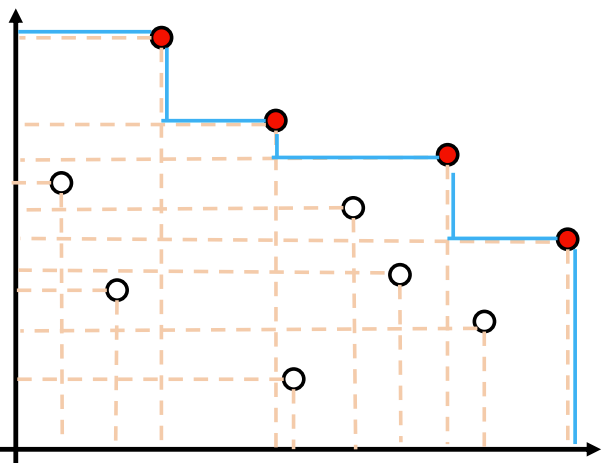
\includegraphics[width=0.25\textwidth]{images/1a.PNG}
                % \caption{}
                \label{fig:1a}
            \end{figure} 

            \item \textbf{Incremental Maxima}: Sort the $n$ distinct (multiple points do not overlap) points of $S$ in descending order by their x-coordinate ($O(n\log n)$). For two points $i, j \in S$, where $i \neq j$, if $i_x = j_x$, then point $i$ comes before $j$ if $i_y > j_y$, and vice versa (order the higher y-coordinate point first). (A) The first point $v$ in the sorted set, $S'$, is trivially in the set of $S$'s maxima, because $v$ has the largest x value (and higher y value against any points with the same x value, which $v$ therefore dominates). Let $m$ be the \emph{latest} maxima found so far, and so, $m_y$ is the current largest y-coordinate; $S'[0]$ is, of course, our first $m$. Checking each point in $S'$ in order, (B) if the current $p$ has a $p_y > m_y$ seen so far, then add $p$ to the set of maxima and make $p$ the new $m$, because our $S'$ ordering has $p_x \leq m_x$, so $m$ doesn't dominate $p$. (C) If the current $p_y \leq m_y$, reject it from the maxima set; since we ordered $S'$ by descending x-coordinate, $p_x \leq m_x$ ($p_y < m_y$ if $p_x = m_x$), $p$ is dominated by $m$. This part of the algorithm runs $O(n)$ time and correctly computes all the maxima of $S$. Space complexity may be $O(1)$ if we sort in place and toss out the points of $S'$ that are not rejected. Overall runtime is $O(n\log n)$ due to preprocessing.
            
            \item \textbf{Divide-and-Conquer Maxima}: Sort the $n$ distinct points of $S$ in ascending order by their x-coordinate, and call it $V$ ($O(n\log n)$). Perform this D\&C operation on $V$, also $O(n\log n)$:
                \begin{enumerate}[label=\arabic*)]
                    \item If $|V| \leq 1$, then return the current set $V$, as it is trivially a set of maxima.
                    \item Otherwise, divide set $V$ evenly into two subsets $L$ and $R$, for the left and right half of the list. Run algorithm from step 1 on $L$ to produce $L'$ (maxima of $L$). Likewise, run it on $R$ to produce $R'$ (maxima of $R$).
                    \item Merge $L'$ and $R'$ to produce maxima set of $V$: All $r \in R'$ are maxima of $V$, because they are the maxima of the right subset; since the set is ordered, no $\ell \in L'$ has a $\ell_x > r_x$ for any $r \in R'$. An $r$ cannot be dominated by an $\ell$. For any $\ell \in L'$ where $\ell_y < R'[0]_y$, discard that $\ell$, because $R'[0]$ (the tallest point in $R'$) dominates $\ell$. Keep only those $\ell$ whose $\ell_y > R'[0]_y$, because those are not dominated by any maxima on the right subset. Return the $L'' \cup R'$ as the maxima set for $V$. 
                \end{enumerate}
                Likewise, space complexity may be $O(1)$ if we sort and do the D\&C in place. Runtime for the D\&C is $O(n\log n)$, $O(\log n)$ divisions and $O(n)$ for the merging. 
            
            \item \textbf{Dynamic Maxima}\footnote{Went over dynamic and MBC algorithm with Jake in office hours, with Alex and Stephanie.}: Sort the $n$ distinct points of $S$ in ascending order by their x-coordinate ($O(n\log n)$). Let these sorted vertices be the leaves of a Balanced Binary Search Tree we shall construct from the leaf level to the root level; the root will contain the maxima of set $S$. At each level of the tree, starting at the leaves, compute the maxima between two adjacent nodes using the strategy described above in part c step 3 when finding the set of maxima between two sets of maxima. Store the resultant maxima set in the parent node of the two adjacent nodes you just compared, in the next level up. Stop when we've computed the root node, which contains maxima of $S$, and is correct using the previous strategy. Since this is a BBST, height of the tree is $O(log n)$, so computing the whole tree was $O(n\log n)$, which works in worst case where every vertex is also a maxima. Insertion and deletion from the BBST as described in class will also be $O(\log n)$ time. And space complexity is $O(n\log n)$ for worst case described previously. 
            
            \item \textbf{Marriage-Before-Conquest Maxima}\footnotemark[1]: Sort the $n$ distinct points of $S$ in ascending order by their x-coordinate ($O(n\log n)$). 
            
                \begin{enumerate}[label=\arabic*)]
                    \item We can compute the median x-line to split the current set into a left $L$ and right $R$ subset in $O(n)$ time. 
                    
                    \item On the $R$ side, we find the max y-coordinate point in $O(n)$ time, we call that point $r_\text{max}$. Using $r_\text{max}$, we can toss out/prune all the points $p$ to the left of $r_\text{max}$ (i.e. all $p$ such that $p_x < r_{\text{max}\ x}$) if $p_y < r_{\text{max}\ y}$, i.e. we prune points which point $r_\text{max}$ can dominate, as they cannot be in the maxima we are computing. Pruning takes $O(n)$ time.
                    
                    \item Repeat from step 1 on whats left of the $L$ and repeat it on what's left of the $R$ side after the pruning. 
                    
                    \item Combine the maxima we found for $L$ and $R$, and report that as the maxima of the current set.
                \end{enumerate}

            Since we can have $O(\log n)$ of these recursions, the overall runtime is $O(n\log n)$. Space complexity is $O(1)$.
        \end{enumerate}
        
    \pagebreak
    % END %%%%%%%%%%%%%%%%%%%%%%%%%%%%%%%%%%%%%%%%%%%%%%%%%%%%%%%%%%%%%%%%%%%

    
    %%%%%%%%%%%%%%%%%%%%%%%%%%%%%%%%%%%%%%%%%%%%%%%%%%%%%%%%%%%%%%%%%%%%%%%%%
    \section{Line Sweep and Augmented Data Structures}
    \label{sec:two}

    Let there be a set $S$ of $n$ disjointed triangles. I have the three vertices of each triangle $t \in S$, as well as their edges. I also have a ``top'' and ``bottom'' edge described by $(x_\text{min} - 1, y_\text{max} + 1), (x_\text{max} + 1, y_\text{max} + 1)$ and $(x_\text{min} - 1, y_\text{min} - 1), (x_\text{max} + 1, y_\text{min} - 1)$, respectively, that partially ``box'' our triangles in a space. These top and bottom edges are perpendicular to the vertical line sweep $\ell$ that sweeps from left to right along the x-axis. I describe a line sweeping method of finding the bridges described in the problem.
        \begin{itemize}
            \item \textbf{Status Data Structure}: A balance binary search tree of edges, where each edge knows the current vertex it ``sees'' at the current point of a sweep. The sweep line $\ell$ starts at the leftmost part of the plane, so only top and bottom edges are inserted into Status, and neither currently see any vertices. Since this is a BBST, insertion and deletion of edges into it will take $O(\log n)$ time. 
            
            % I will show later there is a constant number of these updates to Status, at each vertex visited in Stopping Point, then the algorithm overall runs $O(n\log n)$ time.

            \item \textbf{Stopping Point (SP) Data Structure}: A BBST of vertices of all the triangles of $S$, sorted by x-coordinate. Again, sorting takes $O(n\log n)$ time. In a sweep lining algorithm, I visit each point of the set once. 
            
            % where there can be a constant number of edge updates ($O(\log n)$) in Status.

            \item \textbf{Invariant}: At a current point of the sweep, all bridges to the left of $\ell$ that were found are valid, and all edges in Status currently point to the last vertex they ``see'' in the algorithm. Status only contains edges that $\ell$ intersects.
            
            %%% FIX THIS DEFINITION
            And edge sees a vertex if, at a stage that $\ell$ intersects this vertex, the edge is intersected by $\ell$ and is adjacent to the vertex (there are no edges between this exdge and the vertex). 
        \end{itemize}

        While SP is not empty:
        \begin{enumerate}
            \item Pop a vertex $v$ off of SP. 
            \item If the edges of $v$ are not in Status, add them edge to status and mark that they see $v$ ($O(\log n)$). 
            \item For edges already in Status (i.e. intersected by $\ell$) and it sees a different vertex, update it in status such that the vertex that edge sees is now $v$ ($O(\log n)$). 
            
            There is a constant number of these edge updates at a vertex, because
            
            \begin{enumerate}
                \item  A vertex's own 2 edges always sees it,
                \item an edge on the triangle of the vertex but doesn't contain the vertext and is intersected by $\ell$ directly above or below $v$ would ``see'' $v$ from inside the triangle; *it would already be in Status because it would have been added at a vertex that appeared before $v$,
                \item top and bottom edges \emph{may} also see $v$ since $\ell$ should always intersect top and bottom, 
                \item and at most two edges from other triangle(s) can also see $v$, given that all triangles are disjointed and Status only keeps current edges. Any other additional triangle edges with overlapping x-coordinates would not see $v$ because there is another edge in the way, and those edges with non-overlapping x-coordinates would either already been in and then discarded from Status, or they have not yet been swept and never been in Status.
            \end{enumerate}

            Therefore, for $n$ vertices, where are $O(n\log n)$ to process these vertices.

            \item If, at $v$, two edges in Status were updated to point to $v$, but they were \emph{both} previously pointing to the same vertex $w$, then that means a bridge can be formed between $v$ and $w$. This means there were no other triangles or edges between $v$ and $w$ that a potential bridge could intersect. Some exceptions:
            
                \begin{itemize}
                    \item Checking in constant time, if both vertices belong to the same triangle, that is not a bridge you report. 
                    \item When the vertices belong to different triangles, checking in constant time, if 1 a bridge between the the two triangles already exist, then don't report $\overline{vw}$,
                    \item If we already have $n-1$ bridges, it is not necessary to report $\overline{vw}$.
                \end{itemize}
            
                Report the bridge for $\overline{vw}$, otherwise.
            
            
            
            \item If $v$ is the rightmost point of a triangle, then remove the three edges of the triangle from Status in $O(\log n)$ time.
            \item Repeat at the next stopping point. 
        \end{enumerate}

        Sorting takes $O(n\log n)$ time, visiting each vertex is $O(n)$ time, and processing $n$ vertices each take $O(\log n)$ time for overall $O(n\log n)$ time. Therefore the algorithm takes $O(n\log n)$. Space complexity is $O(n)$ for the SP, and also linear in worst case if all triangles were vertically aligned. 

    \footnote{Jake walked through a correct algorithm for finding these bridges; with Alex and Stephanie.}

        
    \pagebreak
    % END %%%%%%%%%%%%%%%%%%%%%%%%%%%%%%%%%%%%%%%%%%%%%%%%%%%%%%%%%%%%%%%%%%%



    %%%%%%%%%%%%%%%%%%%%%%%%%%%%%%%%%%%%%%%%%%%%%%%%%%%%%%%%%%%%%%%%%%%%%%%%%
    \section{Convex Polygons and Monotone Polygons}
    \label{sec:three}

        \begin{enumerate}[label=\alph*.]
            \item \textbf{Convex Polygon}\footnotemark[2]: When the given vectors are translated to the origin (in the order of a walk around the polygon), the polygon is convex if: 1) the angle given by a vector and the next vector translated must extend in the one direction thats the same as the previous two's direction, i.e. the next vector must not cross over previous vectors added, as this would indicate a two different turns the edges of the polygons take, leading to a concave or complex polygon; and 2) the vectors should only form one rotation around the origin, and cannot continue rotating about the origin more than once, as this corresponse to a polygon that self intersects despite all directed edges forming one kind of turn, as the example in Homework 1.1. Checking this takes $O(n)$ time as we are checking each vector formed by two adjacent vertices.
            
            \item \textbf{Monotone Polygon}\footnote{Discussed verification of these using vectors with Diane and Jake at office hours.}: The following alorithm can run in $O(n)$ time to see if polygon $P$ with $n$ vertices is monotone: 
            
                \begin{enumerate}[label=\arabic*)]
                    \item Take an arbitrary vector starting point $v_0$ to point $v_{1}$, translate that vector to the origin.  
                    \item For each point $v_i \in P$ for $i \in [1,n]$ in order walking about the edge of $P$, translate vector from $v_{i}$ to $v_{i+1}$ to the origin, and increment the count in area of the plane by 1, as it gets swept over by the angle formed by vectors $\overrightarrow{v_{i-1} v_{i}}$ and $\overrightarrow{v_{i} v_{i+1}}$. I call these areas we increment on slices. This takes $O(n)$ time to translate and ``sweep'' all the vectors. 
                        \begin{enumerate}
                            \item To save space and make space complexity constant, we can toss out the slices that have a count greater than 2, as a line of monotonicity cannot lie perpendicular to anything in that area.\footnote{Diane discussed space efficiency about these regions at office hours Alex and Stephanie.} 
                        \end{enumerate}

                    \item We look for these area slices with a count of only 1. If there are at least two of these slices and a straight line $\ell$ can intersect both slices across the origin, then $\ell$ is the line perpendicular to the line of monotonicity of $P$ and so $P$ is montone. It also takes $O(n)$ to look at all the slices, so overall runtime is $O(n)$, and space complexity is constant if we prune. 
                \end{enumerate}

        \end{enumerate}

    \pagebreak
    % END %%%%%%%%%%%%%%%%%%%%%%%%%%%%%%%%%%%%%%%%%%%%%%%%%%%%%%%%%%%%%%%%%%%



    %%%%%%%%%%%%%%%%%%%%%%%%%%%%%%%%%%%%%%%%%%%%%%%%%%%%%%%%%%%%%%%%%%%%%%%%%
    \section{DCEL}
    \label{sec:four}

    \begin{enumerate}
        \item Like how we learnt in class, we can compute the intersection points of two convex polygons in $O(n)$. 
        \item Ignore regions of $P_2$ that exist outside the convex hulls intersections. 
        \item Use an algorithm similar to one described in our text book\footnote{Section 2.1 describes a sweep line algorithm that is used in an algorithm in Section 2.3 for recomputing the half edges of an overlay of two subdivisions, page 34-35 \cite{berg08}.}. In essence, wherever an edge of $P_2$ intersects $P_1$, we locally recompute the DCEL for $P_1$ to include this new local edge. Since $P_1$ is already triangulated, any triangle intersected by a line forms another triangle and a quadrilateral. We can ignore retriangulation, as it is not necessary. Since we are inserting new edges locally into where they intersect $P_1$, making these updates is constant time, and there s $O(n)$ insertions\footnote{Diane went over two versions of this solution in detail at office hours, and I try to describe a version of it here.}. In addition to adding these edges, since the DCEL of $P_1$ gives us information about the faces of the polygon, we can add more attribute information to the new faces affected by the new edge insertions, namely, if a face is an overlap of an interior region of $P_2$ and interior region of $P_1$, and overlap of an interior region of $P_2$ and exterior region (pocket) of $P_1$.
        
        \item At this point, we can conclude that we have all points of $P_2$ that intersects $P_1$. Now we can walk along the edge of $P_2$ and find the areas that represent the $P_1 \cap P_2$. At a point on $P_2$, which may be an intersection point or point of a new edge in the DCEL, start walking along the edges of $P_1$ where which the the face the edge is connected to is marked as being overlapped by an interior region of $P_1$ and $P_2$. If we return to the starting point, report this polygonal intersection. If there are still points on the bounds of $P_2$ we have not reported, go to the next one, and repeat the above procedure. Repeat until we've seen all marked intersection points on the bounds of $P_2$. We have report all the intersections of $P_1 \cap P_2$.
    \end{enumerate}

    
        
    % \pagebreak
    % END %%%%%%%%%%%%%%%%%%%%%%%%%%%%%%%%%%%%%%%%%%%%%%%%%%%%%%%%%%%%%%%%%%%




    %%%%%%%%%%%%%%%%%%%%%%%%%%%%%%%%%%%%%%%%%%%%%%%%%%%%%%%%%%%%%%%%%%%%%%%%%
    

    % \pagebreak
    % END %%%%%%%%%%%%%%%%%%%%%%%%%%%%%%%%%%%%%%%%%%%%%%%%%%%%%%%%%%%%%%%%%%%



\begin{thebibliography}{1}
    \bibitem[1]{officehours}Jake and Diane's office hours, classmates: Stephanie, Alex, Anju with homework problem discussions.
    \bibitem[2]{berg08}Mark de Berg, Otfried Cheong, Marc van Kreveld, and Mark Overmars. 2008. Computational Geometry: Algorithms and Applications (3rd ed. ed.). Springer-Verlag TELOS, Santa Clara, CA, USA.
\end{thebibliography}
%%%%%%%%%%%%%%%%%%%%%%%%%%%%%%%%%%%%%%%%%%%%%%%%%%%%%%%%%%%%%%%%%%%%%%
\end{document}
%%%%%%%%%%%%%%%%%%%%%%%%%%%%%%%%%%%%%%%%%%%%%%%%%%%%%%%%%%%%%%%%%%%%%%

